\chapter{Systemarkitektur (Alle)}

\section{Version}
\begin{table}[h]
	\centering
	\begin{tabularx}{\textwidth - 2cm}{|l|l|l|X|}
	\hline
	Dato	& Version	& Initialer & Ændring	\\ \hline
	11. marts & 1 & KS & Første udkast. \\ \hline
	18. marts & 2 & MHG & Inden review. \\\hline
	23. marts & 3 & MHG & Rettelser efter review. \\\hline		
	16. april & 4 & MHG & Rettet til så \IIC sensorer forsynes fra MasterPSoC. \\\hline 
	\end{tabularx}
\end{table}

\section{Indledning}

I dette kapitel vil systemarkitekturen for AutoGreen være opdelt i to underdele, hhv. for hardware og for software. Formålet med kapitlet er at gøre systemets grænseflader, både interne og eksterne, klare ift. signaltyper, niveauer og softwaregrænseflader.

\section{Hardwarearkitektur}
Dette afsnit beskriver arkitektur for hardware i AutoGreen.

Forsyning til alle blokke er beskrevet på IBD for system, Figur \ref{fig:ibd_system_forsyn}. Forsyninger er ikke tegnet ind på øvrige diagrammer for overskuelighedens skyld. Det gælder desuden at alle blokke har fælles reference (GND). 

\clearpage

\subsection{BDD for System}
\begin{figure}[h]
\centering 
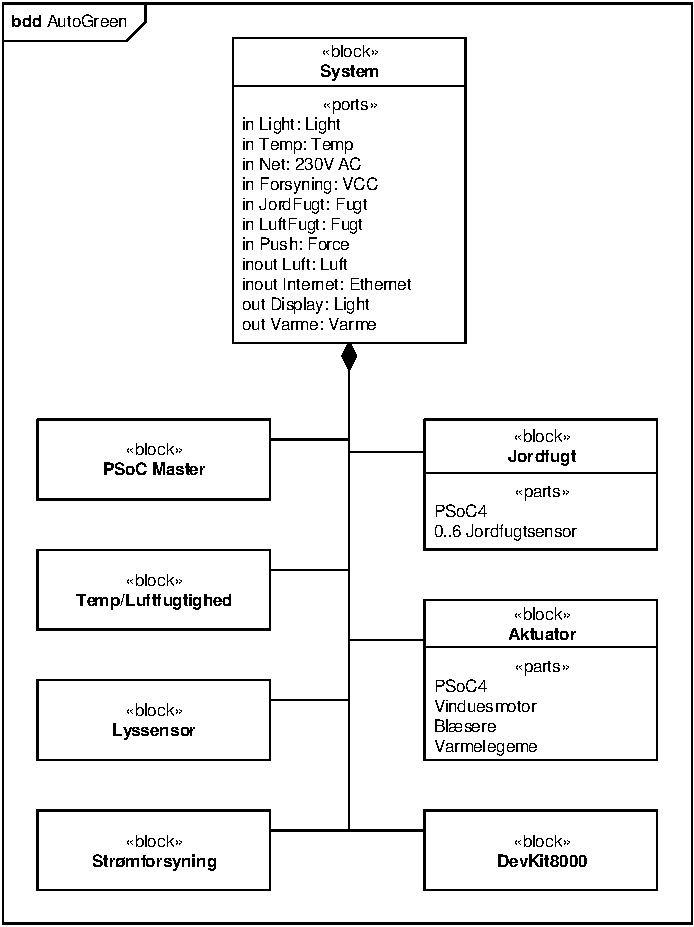
\includegraphics[width={\textwidth-2cm}, trim=0 0 0 0, clip=true] {../fig/bdd_system.pdf}
\caption{BDD for System.}
\label{fig:bdd_system}
\end{figure}

\clearpage

\subsection{IBD'er for System}

\begin{figure}[!h]
\centering 
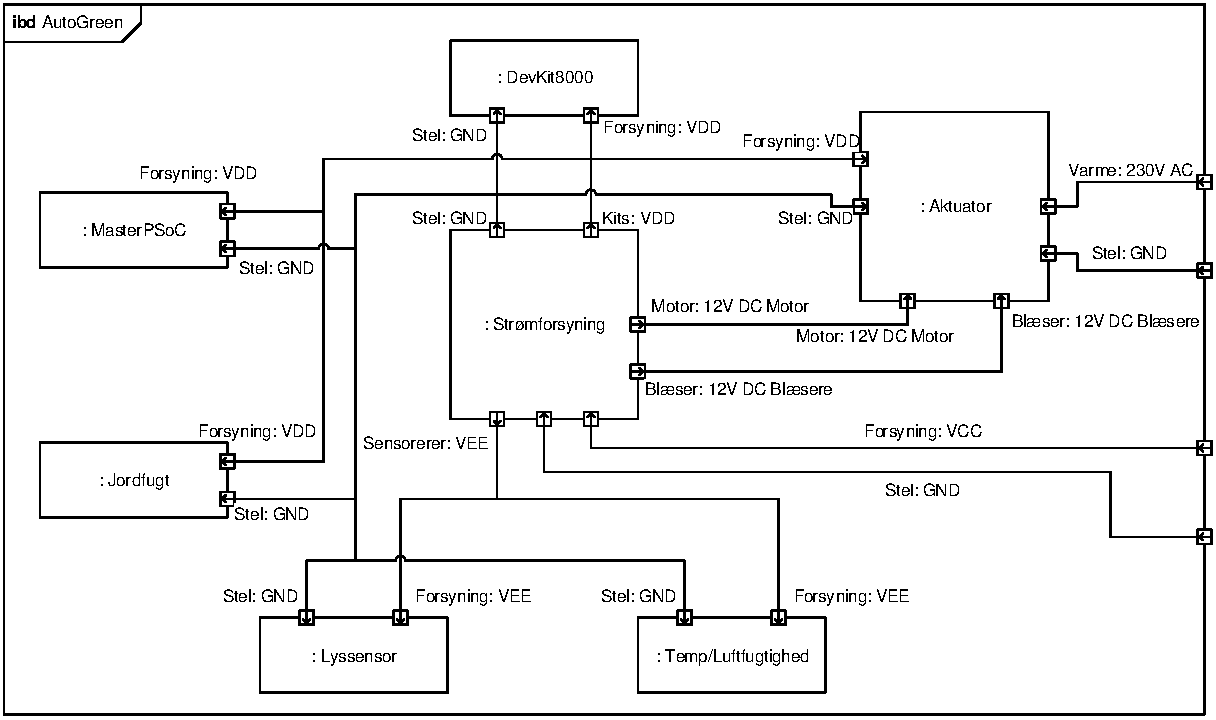
\includegraphics[width={\textheight-65 pt}, angle = 90] {../fig/ibd_system_forsyninger.pdf}
\caption{IBD for forsyninger i systemet.}
\label{fig:ibd_system_forsyn}
\end{figure}

\clearpage

\begin{figure}
\centering 
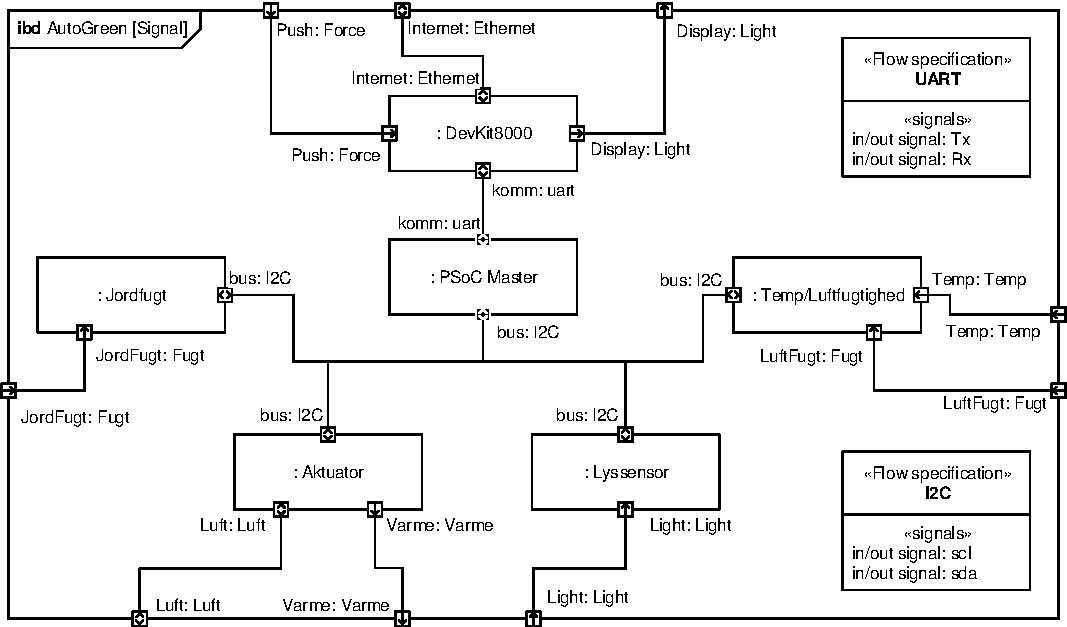
\includegraphics[width={\textheight-25 pt}, angle = 270] {../fig/ibd_system_signaler.pdf}
\caption{IBD for signaler i systemet.}
\label{fig:ibd_system_signal}
\end{figure}

\clearpage

\subsubsection{Strømforsyning}
Forsyner øvrig hardware i systemet, undtagen varmelegemet, Devkit8000 samt sensorer. Blokken forsynes fra en laboratorieforyning.
\subsubsection{DevKit8000}
Systemets brugerflade, er samtidigt controller for systemet. 
\subsubsection{PSoC Master}
PSoC4 Pioneer Kit, der har til opgave at kommunikere via UART med DevKit8000 og via \IIC med slaver.  
\subsubsection{Temp/Luftfugtighed}
Denne blok indeholder en sensor med \IIC interface og måler temperatur og luftfugtighed i det fysiske drivhus.
\subsubsection{Lyssensor}
Består af en sensor med \IIC interface og måler lysintensitet i det fysiske drivhus. 
\subsubsection{Jordfugt}
Denne blok indeholder op til seks analoge jordfugtsensorer, som vha. et PSoC4 Pioneer Kit er koblet på systemets \IIC bus.
\subsubsection{Aktuator}
Denne blok indeholder et PSoC4 Pioneer Kit, der fungerer som \IIC slave og styrer systemets aktuatorer. 

\clearpage

\subsection{IBD for Aktuator}

\begin{figure}[h]
\centering 
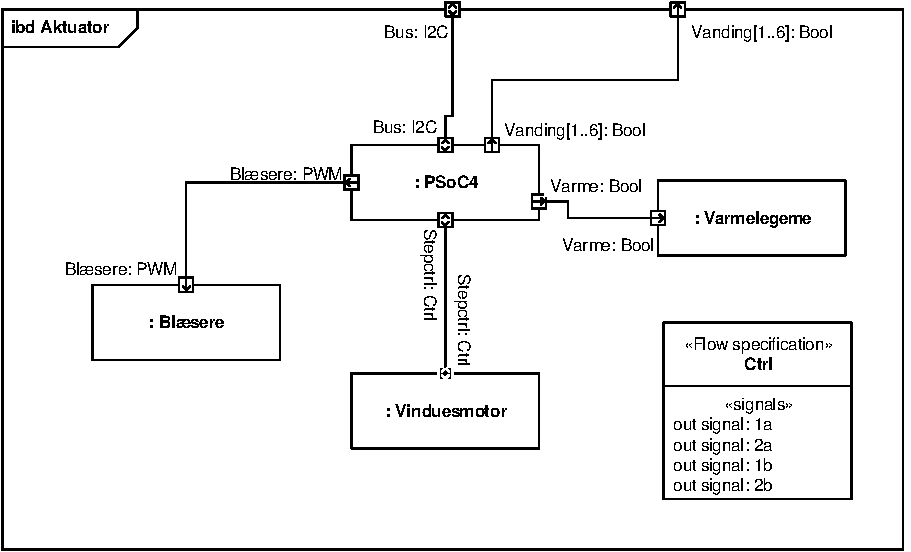
\includegraphics[width={\textwidth}, trim=0 0 0 0, clip=true] {../fig/ibd_aktuator.pdf}
\caption{IBD for Aktuator}
\label{fig:ibd_aktuator}
\end{figure}

\subsubsection{PSoC4}
PSoC blokken består af et PSoC4 Pioneer Kit, der agerer slave på \IIC bussen. 
\subsubsection{Vinduesmotor}
Denne blok består af en steppermotor, der styrer vinduet i det fysiske drivhus.
\subsubsection{Varmelegeme}
Varmelegeme med formål at hæve temperaturen i det fysiske drivhus. Varmelegemet styres af PSoC4 blokken, og det forsynes direkte fra elnettet (230V AC). 
\subsubsection{Blæsere}
Denne blok består af fire blæsere, som kan ventilere luften i det fysiske drivhus. Blæserne styres af PSoC4, og de forsynes fra Strømforsyning. 

\clearpage

\subsection{IBD for Jordfugt}

\begin{figure}[h]
\centering 
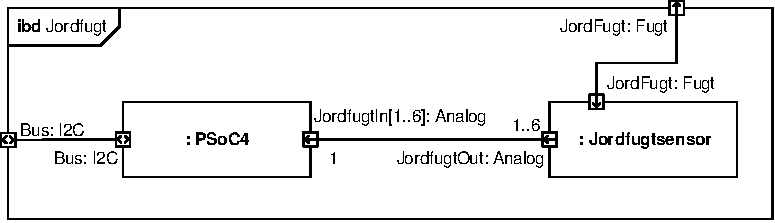
\includegraphics[width={\textwidth}] {../fig/ibd_jordfugt.pdf}
\caption{IBD for Jordfugt}
\label{fig:ibd_jordfugt}
\end{figure}

\subsubsection{PSoC4}
PSoC4 Pioneer Kit, der agerer slave på \IIC-bussen. 
\subsubsection{Jordfugtsensor}
Denne blok indeholder en analog sensor, der måler jordfugt ved en plante i det fysiske drivhus. Der kan kobles op til seks af disse til PSoC4.

\clearpage

\subsection{Signalbeskrivelser}
\label{subsec:signalbeskrivelser}

%\LTXtable{\textwidth}{Systemarkitektur/HWarkitektur/signalbeskrivelser.tex}

\begin{table}[h]
\begin{tabularx}{\textwidth}{| l | >{\raggedright}X | >{\raggedright}X | >{\raggedright\arraybackslash}X |>{\raggedright}X |}
\hline
	\textbf{Signaltype} & \textbf{Funktion} & \textbf{Tolerancer} & \textbf{Kommentar}\\ \hline
	VCC & Forsyning til strømforsyning & 12V $\pm$ 0,25V \newline 3A max. & Lab.forsyning  \\\hline	
	VDD & Forsyning til alle PSoC4 Pioneer Kits. & 5V DC $\pm$ 0.15V, \newline 0.5A max & - \\\hline
	VEE & Forsyning til sensorer & 3.3V DC $\pm$ 0.1V, \newline 0.1A max & - \\\hline
	12V DC Blæsere & Forsyning til blæsere. & 12V DC $\pm$ 0,25V, \newline 140mA max. & - \\\hline	
	12V DC Motor & Forsyning til vinduesmotor. & 12V $\pm$ 0,25V, \newline 500mA max. & - \\\hline
	230V AC & Forsyning til varmelegeme og DevKit8000. & 230V AC $\pm$ 10\%, \newline 50 Hz, \newline 0.3A max & - \\\hline
	Analog & Analogt målesignal fra jordfugtmåler. & 0-3.3V $\pm$ 0.1V & - \\\hline	
	Bool & Digitalt signal til styring af vanding og varmelegeme. & 0-3.3V & 1=True: 2.8-3.3V \newline 0=False: 0-0.4V \\\hline	
	Ctrl & Styring af stepper motor & 0-3.3V & 1=True: 2.8-3.3V \newline 0=False: 0-0.4V  \newline Består af fire signaler: \newline 1a, 2a, 1b, 2b \\\hline	
	GND & Stel & 0V & Reference \\\hline	
	I2C & Kommunikation mellem \IIC enheder. & 0-3.3V & 1=True: 2.8-3.3V \newline 0=False: 0-0.4V \newline Består af to signaler: \newline sca og scl \\\hline	
	UART & Kommunikation mellem DevKit8000 og Master & 0-5V & 1=True: 4.5-5V \newline 0=False: 0-0.4V \newline Består af 2 signaler: \newline Tx og Rx \\\hline	
	PWM & Styring af blæsere vha. pulsbreddemodulation. & 0-3.3V \newline 1 kHz & Duty cycle styres fra 0-100\% i trin fra 0-255. 0 svarer til 0\% og 255 svarer til 100\% \\\hline
\end{tabularx}
\caption{Beskrivelse af signaler.}
\label{tbl:signalbeskriv}
\end{table}

\clearpage

\section{Softwarearkitektur}

\subsection{Applikationsmodel}

Applikationsmodellen er valgt ud fra udviklernes synspunkt og bruges for at give overblik over hvilke klasser som skal laves, og hvilket ansvar de hver især har. Nedenstående UML skal ses som det overordnede system og menuklasserne er udeladt for at skabe overblik. 

\begin{figure}[!h]
\centering 
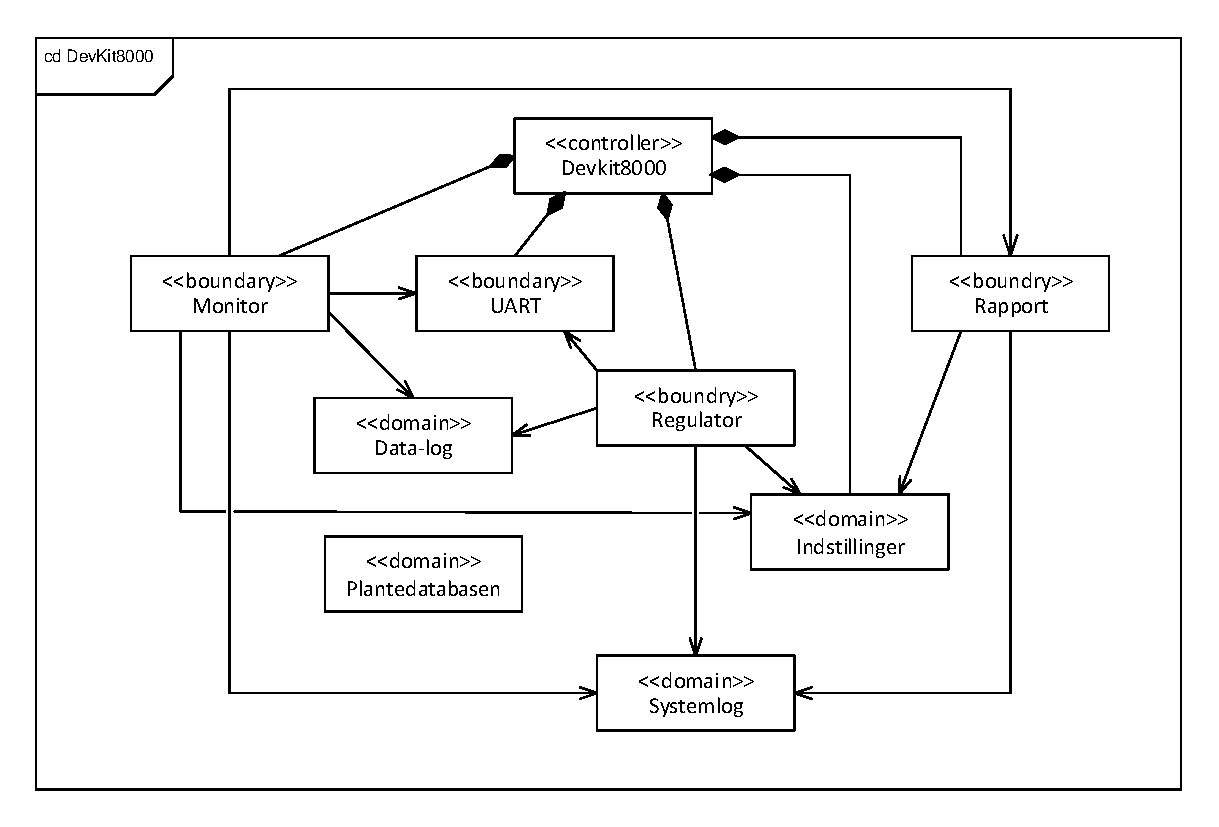
\includegraphics[scale=0.8] {../fig/UML_autogreen.pdf}
\caption{Application model for AutoGreen}
\label{fig:UML}
\end{figure}

\subsection{Controller-Klasser}

\subsubsection{DevKit8000}

DevKit8000 klassen skal initiere systemet og har derfter ansvaret for styring af processerne Regulering og Monitoring.
DevKit8000 klassen indeholder alle menuer beskrevet i menuoversigt. Brugeren kan interagere med klassen igennem menuerne.
Controller-klassen har igennem menuerne set i menuoversigten tilgang til de andre klasser i systemet.

\subsection{Boundary-Klasser}

\subsubsection{Monitor}

Monitorklassens primære opgave er at opsamle sensordata fra UART klassen og skrive dem til data-loggen. Der ud over skal Monitor skrive til System-log, hvis UART klassen rapporterer fejl ved dataoverførelse.

\subsubsection{Regulator}

Reguleringsklassen har ansvaret for at planterværdierne bliver overholdt. Den opnår dette ved at læse fra data-loggen, samt indstillinger som indeholder de virtuelle planter og hvis uregelmæssigheder findes blandt disse data, vil klassen tænde de fornødende akutuatorer gennem UART klassen. Der ud over skal Regulator skrive til System-log, hvis UART klassen rapporter fejl ved data overførelse.

\subsubsection{UART}

UARTklassen er grænsefladen mellem Devkittet og de sensorer/akutuatorer, der måtte eksistere i AutoGreen systemet.

\subsubsection{Rapport}

Rapportering indlæser E-mailkonfigurationer fra indstillinger, som bestemmer hvilken slags E-mails, der skal benyttes. Rapporting skal sende E-mail til brugeren dagligt, når der er kritisk klima i drivhuset, eller både dagligt og ved kritisk klima.

\subsection{Domain-Klasser}

\subsubsection{Data-log}

Data-loggen styrer en datastruktur. Det er dens opgave at modtage og indsætte målte data from drivhusklima i datastrukturen, samt hente informationer ud fra strukturen.

\subsubsection{System-log}

System-loggen har til ansvar at styre en datastruktur med henblik på at gemme de vigtigste systemhændelser og skal kunne tilgåes af brugeren senere.

\subsubsection{Indstillinger}

Indstillinger gemmer konfigurationer og indlæser dem i konfigurationsfilen, når regulering eller rapportering startes af brugeren. Den holder gemmer også de virtuelle planter og hvilken hardware der må bruges til at regulere temperaturen med. Der ud over bruges den også til at indstille og hente tiden i systemet.

\subsubsection{Plantedatabasen}

Plantedatabasen gemmer parametre for brugerdefinerede planter samt prækonfigurede planter og tilgås via en klasse menu.

\clearpage

\subsection{Menuoversigt}

Menuoversigten giver et overblik over de forskellige menuer og hvilke menuer, der giver tilgang til hinanden.

\begin{figure}[!h]
\centering 
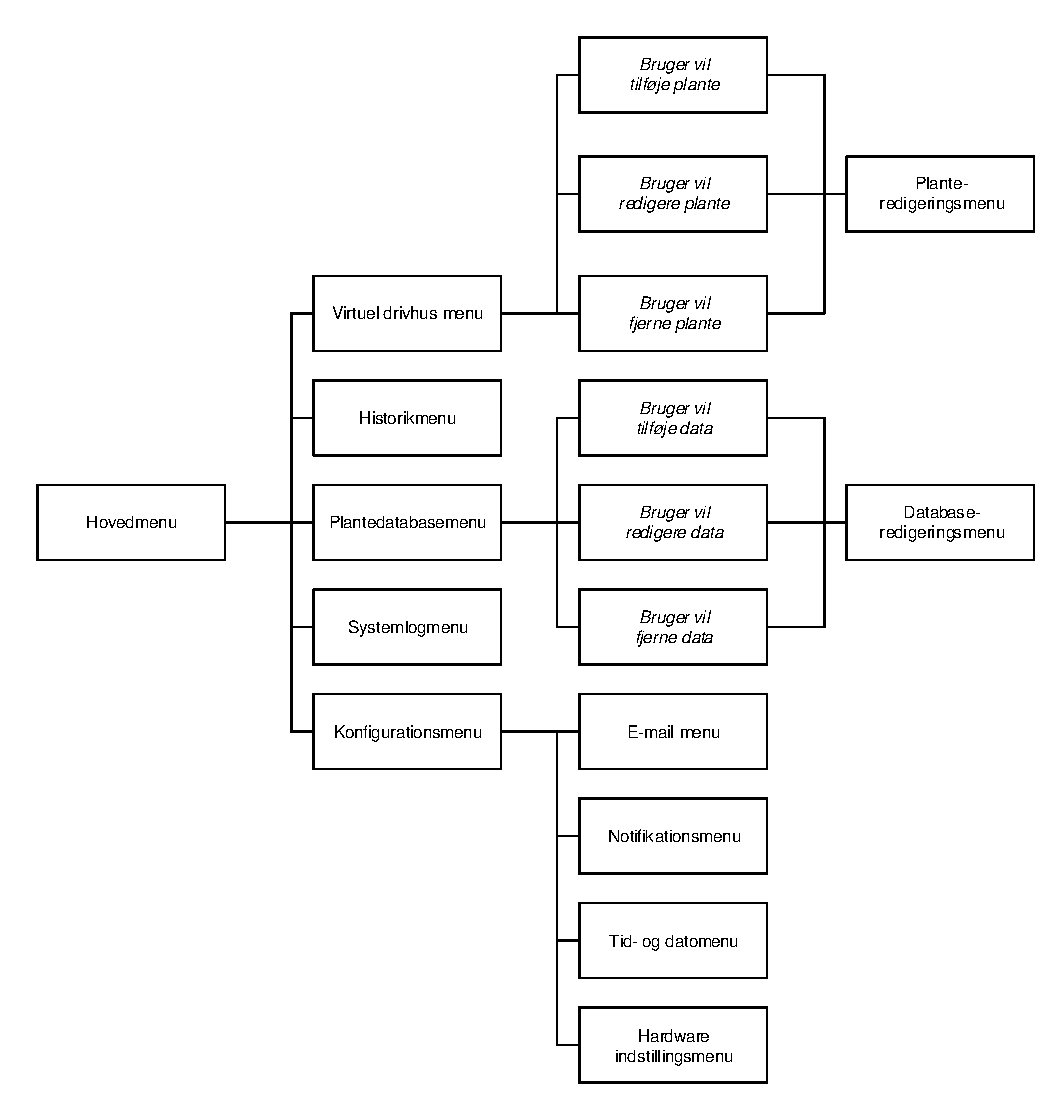
\includegraphics[scale=0.7] {../fig/menu_oversigt.pdf}
\caption{Oversigt over AutoGreen's menuer}
\label{fig:QTMenu}
\end{figure}

\subsection{Menubeskrivelse}
Menuoversigten er med til at give et overblik over hvordan de forskellige menuer tilgåes igennem systemet, og fra hvilke menuer man kan tilgå andre menuer. Hovedmenuen er som standard stedet, hvor brugeren starter, da er her muligt at monitorere drivhusklimaet. I hovedmenuen har brugeren mulighed for at tilgå de 5 undermenuer: virtuel drivhus-, historik-, plantedatabase-, systemlog- og konfigurationsmenu.

\subsubsection{Virtuelle drivhusmenu}
I det virtuelle drivhus har brugeren mulighed for at tilføje nye planter til drivhuset, redigere allerede tilstedeværende planter, og herunder slette planter fra drivhuset. Uanset ønsket skal brugeren tilgå planteredigeringsmenuen.

\subsubsection{Historikmenu}
I historikmenuen har brugeren mulighed for at se data over drivhuset op til et år tilbage.

\subsubsection{Plantedatabasemenu}
I plantedatabasemenuen har brugeren mulighed for at tilføje nye planter til databasen. Ved tryk på 'tilføj plante' oprettes en ny tom virtuel plante i databasen. Denne virtuelle plante åbnes i databaseredigeringsmenuen, hvor dens paramentre kan indstilles efter behov. Hvis brugeren ønsker at redigere allerede oprettede planter eller slette disse, kan brugeren trykke på den ønskede plante. Den valgte plante vil blive åbnet gennem databaseredigeringsmenuen, og det er her muligt at redigere eller slette planten.

\subsubsection{Systemlogmenu}
I systemloggen har brugeren mulighed for at se systemhændelser, f.eks. hvis systemet vælger at åbne et vindue, starte en blæser, eller bruge varmelegemet.

\subsubsection{Konfigurationsmenu}
I konfigurationsmenu har brugeren mulighed for at tilgå 4 undermenuer: E-mailmenu, Notifikationsmenu, Tid- og datomenu, samt Hardware Indstillingsmenu.

\subsubsection{E-mailmenu} \label{sec:mailmenu}
I E-mailmenuen, vises 3 kolonner, hvor brugeren har mulighed for at indtaste E-mail adresse, som skal modtage notifiktationer. 

\subsubsection{Notifikationsmenu} 
I notifikationsmenuen har brugeren mulighed for at slå notifikationer til og fra for både advarsels-notifikationer og daglige notifikationer. 

\subsubsection{Tids- og datomenu} 
I Tids- og datomenuen har brugeren mulighed for at ændre dato og tid. 

\subsubsection{Hardware Indstillingsmenu} 
I Hardware Indstillingsmenu har brugeren mulighed for at vælge hvilke akutuatorer drivhuset skal bruge. Hvis brugeren ønsker at spare strøm, kan blæser og varmelegeme fravælges til regulering temperaturen.

\clearpage

\clearpage
\section{Protokol for UART} \label{UART_Protokol} %TODO Skift dette label ud med 'sec:UART_protokol' her og i samtlige steder den bliver brugt :)

I projektforløbets senere faser deles arbejdet op mellem en HW- og en SW-gruppe. SW gruppen har ansvar for design og implementering af SW på DevKit8000, mens HW gruppen har ansvar for design og realisering af HW og SW på PSoC4 Pioneer Kits. UART kommunikationen mellem PSoC Master og DevKit8000 defineres derved som grænsefladen mellem HW og SW, omend en del af funktionaliteten på PSoC4 Pioneer Kits realiseres vha. SW.

\subsection{UART indstillinger}

\begin{itemize}
\item Baud rate: 9600 
\item Antal bits: 8
\item Antal stop bits: 1
\item Paritet: Even
\end{itemize}

\subsection{Datavalidering}

For at sikre validering af data sendt fra DevKit8000 til PSoC4 Master, sendes der altid svar tilbage fra PSoC4 Master til DevKit8000. Svaret består af en gentagelse af den modtagne kommando og evt. nogle dataværdier. \newline
Såfremt der går noget galt i I2C kommunikationen i HW delen af systemet, sendes en fejlkode til DevKit8000. 
Derved er der mulighed for at SW på DevKit8000 kan logge fejlhændelser i systemloggen, og fx gensende kommandoer eller kassere data. \newline
Da hver enkelt byte, der sendes via UART er vedlagt en paritetsbit sikrer vi os til dels at hver byte overføres korrekt. \newline
Når DevKit8000 sender en kommando via UART skal PSoC Master svare indenfor 2 sekunder. Såfremt dette ikke sker, sendes kommandoen igen mindst to gange. Alle kommandoer udføres serielt, hvilket vil sige at næste kommando ikke sendes før der er modtaget svar på den foregående.

\subsection{Kommandoer}

\LTXtable{\textwidth}{Systemarkitektur/UARTprotokol/kommandoer}

